\documentclass{report}
\usepackage[utf8]{inputenc}
\usepackage[T1]{fontenc}
\usepackage{graphicx}
\usepackage[francais]{babel} 
\usepackage{array} 

\title{Etat de l'art}
\author{Projet DUT INFO}
\date{17 Septembre 2013}
\begin{document}
\maketitle
\tableofcontents

\part{Introduction}

\chapter{Principe d'affichage d'une image sur ordinateur}
<<<<<<< HEAD
=======
\section{Introduction}
>>>>>>> f5678a064e854107831d2ce6877a0fd4e21291a1


\chapter{OpenGL}

\section{Introduction}
Comme vu précédemment l'affichage de contenu à l'écran par ordinateur consiste en un processus de communication entre le processeur , la carte graphique et l'écran.Ces messages, très bas niveau, sont difficilement utilisables directement par les développeurs.

OpenGL est une Interface de Programmation (API) qui définit un moyen de communication entre l'application et la carte graphique.
Cependant il n'existe aucune implémentation "officielle" d'OpenGL, c'est le rôle de chaque constructeur de l'implémenter sur son matériel.  
Elle contient un ensemble de 150 fonctions qui permettent de définir les objets et opérations nécessaires pour rendre un contexte tri-dimensionnel.
L’avantage d'OpenGL est qu’elle est totalement portable avec tous les systèmes d'exploitation. Ceci est dû au fait qu'elle sert plutôt d'intermédiaire entre l'application et le système d'exploitation. OpenGL sert à faire le rendu et le communiquer à la carte graphique mais ne gère ni le fenêtrage, ni les événements. 
La majorité des bibliothèques graphiques utilisées pour créer des fenetres graphiques gèrent OpenGL, il est donc possible d'utiliser OpenGL dans un contexte SDL, SFML, QT, API Windows.

%Device context ? Rendering context ?

OpenGL est basé sur un principe de primitives : chaque objet est composé de primitives (sommets, faces, polygones) Pour créer un objet, il suffit donc de définir toutes ses primitives

\newcolumntype{M}[1]{>{\raggedright}m{#1}}

\begin{center}
   \begin{tabular}{| c | M{8cm} |}
   	 \hline
     \verb|GL_POINTS| 			& Dessine un point à chaque n vertex  \tabularnewline
     \hline
     \verb|GL_LINE| 			& Dessine une ligne d’un point n à n+1 \tabularnewline
     \hline
     \verb|GL_LINE_STRIP| 		& Dessine un ensemble de lignes connectées d’un vertex à un autre \tabularnewline
     \hline
     \verb|GL_LINE_LOOP| 		& Même chose que \verb|GL_LINE_STRIP|, mais du dernier vertex, on revient au premier. \tabularnewline
     \hline
     \verb|GL_TRIANGLES| 		& Dessine des triangles avec 3 vertex \tabularnewline
     \hline
     \verb|GL_TRIANGLE_STRIP| 	& Dessine une série de triangles avec les n vertexs définis   \tabularnewline
     \verb|GL_TRIANGLE_FAN| 	& Même chose que \verb|GL_TRIANGLE_STRIP|, sauf que le sommet de chaque triangle est le premier vertex défini \tabularnewline
     \hline
     \verb|GL_QUADS| 			& Dessine un quadrilatère avec 4 vertex \tabularnewline
     \hline
     \verb|GL_QUAD_STRIP| 		& Dessine une série de quadrilatères avec les n vertex définis \tabularnewline
     \hline
     \verb|GL_POLYGON| 			& Dessine un polygône générique dont le nombre de segments \verb|n’est| pas prédéterminé \tabularnewline
     \hline
   \end{tabular}
 \end{center}
 
     \begin{center}
     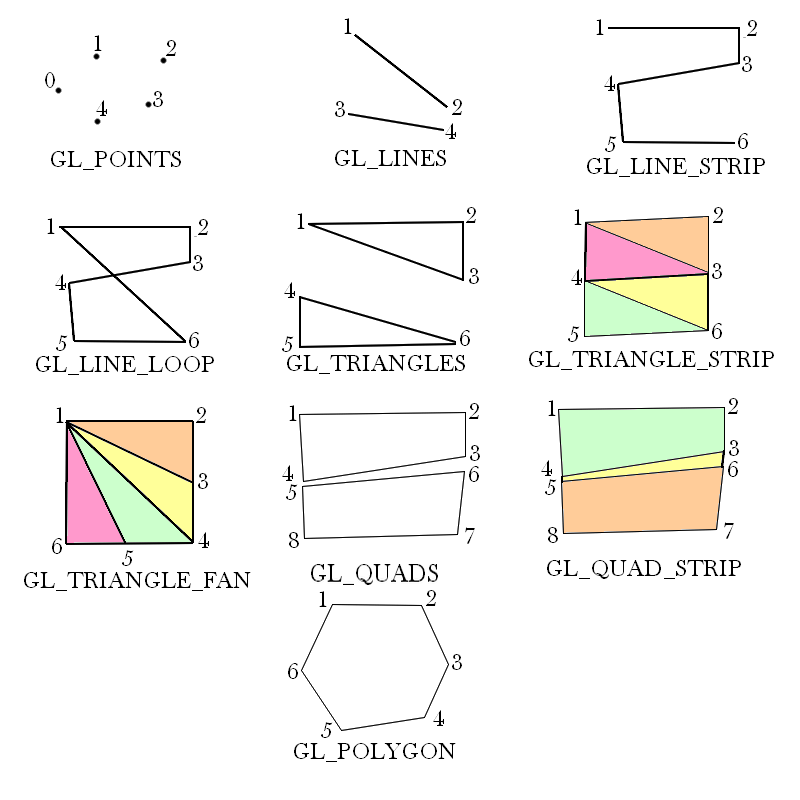
\includegraphics[height=11cm]{img/Primitives}
    \end{center}
\newpage

\section{Fonctionnement d'OpenGL}


%A compléter

\newpage

\chapter{Bibliothèque de rendu 3D}

%A compléter

\newpage
\end{document}